\documentclass{article}


\usepackage{arxiv}

\usepackage{placeins}
\usepackage[utf8]{inputenc} % allow utf-8 input
\usepackage[T1]{fontenc}    % use 8-bit T1 fonts
\usepackage{hyperref}       % hyperlinks
\usepackage{url}            % simple URL typesetting
\usepackage{booktabs}       % professional-quality tables
\usepackage{amsfonts}       % blackboard math symbols
\usepackage{nicefrac}       % compact symbols for 1/2, etc.
\usepackage{microtype}      % microtypography

\usepackage{graphicx}	% to insert graphs
\usepackage{caption}	% to customize caption style
\usepackage{float}
\usepackage{subfigure}

\usepackage{amsmath}

\title{COMP0037 ASSIGNMENT 3}


\author{
 Group: \texttt{Group L}\\\\
 \textbf{Members:} \texttt{Yun Fang, Yusi Zhou}
}

%\date{}

\begin{document}

\maketitle

\captionsetup[figure]{labelformat={default},labelsep=period,name={Fig.}}

% -------------------------------------------------------------------------------------------
\section{Decision Re-Plan Policy}

Let $T_{W}$ be the time the robot has to wait after the obstacle has been discovered.

Note that:

$T$ is the number of timesteps the obstacle remains in front of the robot. 

$L_{W}$ is the cost of waiting a timestep.

% ------------------
\subsection{}

Let $B_{1}$ be the cell where the robot first detects the obstacle.
If the robot decides it will wait, then on average the path cost of waiting at aisle B is less than or equal to planning a new path down aisle C. So:
\begin{align*}
\mathbb{E}(L_{B_{1}BG} + \text{waiting cost}) &\leq \mathbb{E}(L_{B_{1}CG})	\\
L_{B_{1}BG} + \mathbb{E}(T_{W}) * L_{W} &\leq L_{B_{1}CG} 	&\quad	&\Leftarrow \text{the path length and $L_{W}$ are constants}	\\
\mathbb{E}(T_{W}) &\leq \frac{L_{B_{1}CG} - L_{B_{1}BG} } {L_{W}}	\\
\frac{1}{\lambda_{B}} &\leq \frac{L_{B_{1}CG} - L_{B_{1}BG} } {L_{W}}	&\quad	&\Leftarrow  \mathbb{E}(T_{W}) = \mathbb{E}(T) = \frac{1}{\lambda_{B}} \\
\lambda_{B} &\geq \frac {L_{W}} {L_{B_{1}CG} - L_{B_{1}BG} } 	\\
\end{align*}

Therefore, the smallest value of $\lambda_{B}$ on average that waiting is the better strategy is $ \frac {L_{W}} {L_{B_{1}CG} - L_{B_{1}BG} } $.

% ------------------
\subsection{}

If starting at I and the robot decides to drive down aisle C directly, then on average the path cost via B is greater than that via C, so:
\begin{align*}
\mathbb{E}(L_{IBG} + \text{waiting cost}) &> \mathbb{E}(L_{ICG})	\\
L_{IBG} + \mathbb{E}(T_{W}) * L_{W} &> L_{ICG} 	&\quad	&\Leftarrow \text{the path length and $L_{W}$ are constants}	\\
\mathbb{E}(T_{W}) &> \frac{L_{ICG} - L_{IBG} } {L_{W}}	\\
\frac{1}{\lambda_{B}} &> \frac{L_{ICG} - L_{IBG} } {L_{W}}	&\quad	&\Leftarrow  \mathbb{E}(T_{W}) = \mathbb{E}(T) = \frac{1}{\lambda_{B}} \\
\lambda_{B} &< \frac {L_{W}} {L_{ICG} - L_{IBG} } 	\\
\end{align*}

Therefore, the maximum value of $\lambda_{B}$ at which the robot will decide to drive directly down C is $\frac {L_{W}} {L_{ICG} - L_{IBG} } $.

% ------------------
\subsection{}
The event that the robot has to wait after the obstacle has been discovered is now separated into two case: one is the obstacle presents, which has the probability $p_{B}$, and the robot remains alive for T time steps; the other one is the obstacle does not presents, which has the probability $(1-p_{B})$. And in the latter case the time that the robot remains alive is 0. Due to that the event the obstacle presents or not and that the time the obstacle remains active are independent, $T_{W} = p_{B}*T + (1-p_{B}) * 0 = p_{B}*T $.

Then $\mathbb{E}(T_{W}) = \mathbb{E}(p_{B}*T) =p_{B} * \mathbb{E}(T)  = p_{B} / \lambda_{B}$. \\


If the the robot attempt to drive aisle B first, then it means:
\begin{align*}
\mathbb{E}(L_{IBG} + \text{waiting cost}) < \mathbb{E}(L_{ICG})	\\
\end{align*}

Similarly, we can obtain that:
\begin{align*}
\frac{p_{B}}{\lambda_{B}} &< \frac{L_{ICG} - L_{IBG} } {L_{W}}	\\
p_{B} &< \frac{\lambda_{B}  \cdot (L_{ICG} - L_{IBG})}{L_{W}}
\end{align*}

Therefore for a fixed value of $\lambda_{B}$ if the value of $p_{B}$ is below $\frac{\lambda_{B}  \cdot (L_{ICG} - L_{IBG})}{L_{W}}$ the robot will attempt to drive aisle B first.

% ------------------
\subsection{}

In this situation if the robot computes that the path via aisle D is the shortest, it means that:
\begin{align}
\mathbb{E}(L_{IDG}) &< \mathbb{E}(L_{IBG} + T_{WB} * L_{W})	\\
\mathbb{E}(L_{IDG}) &< \mathbb{E}(L_{ICG} + T_{WC} * L_{W})
\end{align}
Where
\begin{align*}
\mathbb{E}(T_{WB}) = p_{B} / \lambda_{B}	\\
\mathbb{E}(T_{WC}) = p_{C} / \lambda_{C}	\\
\end{align*}

By summing (1) and (2) together:
\begin{align*}
2 \cdot \mathbb{E}(L_{IDG}) &<  \mathbb{E}(L_{IBG} + T_{WB} * L_{W}) + \mathbb{E}(L_{ICG} + T_{WC} * L_{W}) \\
2 \cdot L_{IDG} &< L_{IBG} + \mathbb{E}(T_{WB}) * L_{W} + L_{ICG} + \mathbb{E}(T_{WC}) * L_{W}	\\
2 \cdot L_{IDG} &< L_{IBG} + L_{ICG} + L_{W} \cdot (\mathbb{E}(T_{WB}) + \mathbb{E}(T_{WC})) 	\\
2 \cdot L_{IDG} &< L_{IBG} + L_{ICG} + L_{W} \cdot (p_{B} / \lambda_{B}+p_{C} / \lambda_{C}) 	\\\
L_{IDG} &< 0.5L_{IBG} + 0.5L_{ICG} + 0.5L_{W} \cdot (p_{B} / \lambda_{B}+p_{C} / \lambda_{C}) 	\\
\end{align*}

Therefore, if the path via aisle D is the shortest path then the upper bound on the value of the path length is $0.5L_{IBG} + 0.5L_{ICG} + 0.5L_{W} \cdot (p_{B} / \lambda_{B}+p_{C} / \lambda_{C}) $.


\newpage
% -------------------------------------------------------------------------------------------
\section{Implement System in ROS}

% ------------------
\subsection{}

We first add a function in the class which returns a cell coordinate as the intermediate destination, according to the aisle passed in. Then in the \textit{planPathToGoalViaAisle()}, we call this function to get the intermediate cell coordinate and search a path from the given start cell to the intermediate cell. If there was a path then we extract and store this path and then search the second path which is from the intermediate cell to the given goal cell. If the second path existed, we extract it and link it to the first one using the provided function \textit{addToEnd()}. At the end of this function we call the \textit{searchGridDraw} to show the first path so that the two paths can be seen simultaneously.


The result is shown in Fig. \ref{performance2.1}. The start point is marked purple, the intermediate cell is marked green, and the goal is marked blue.

\begin{figure}[H]
\centering  
\subfigure[Via Aisle A]{
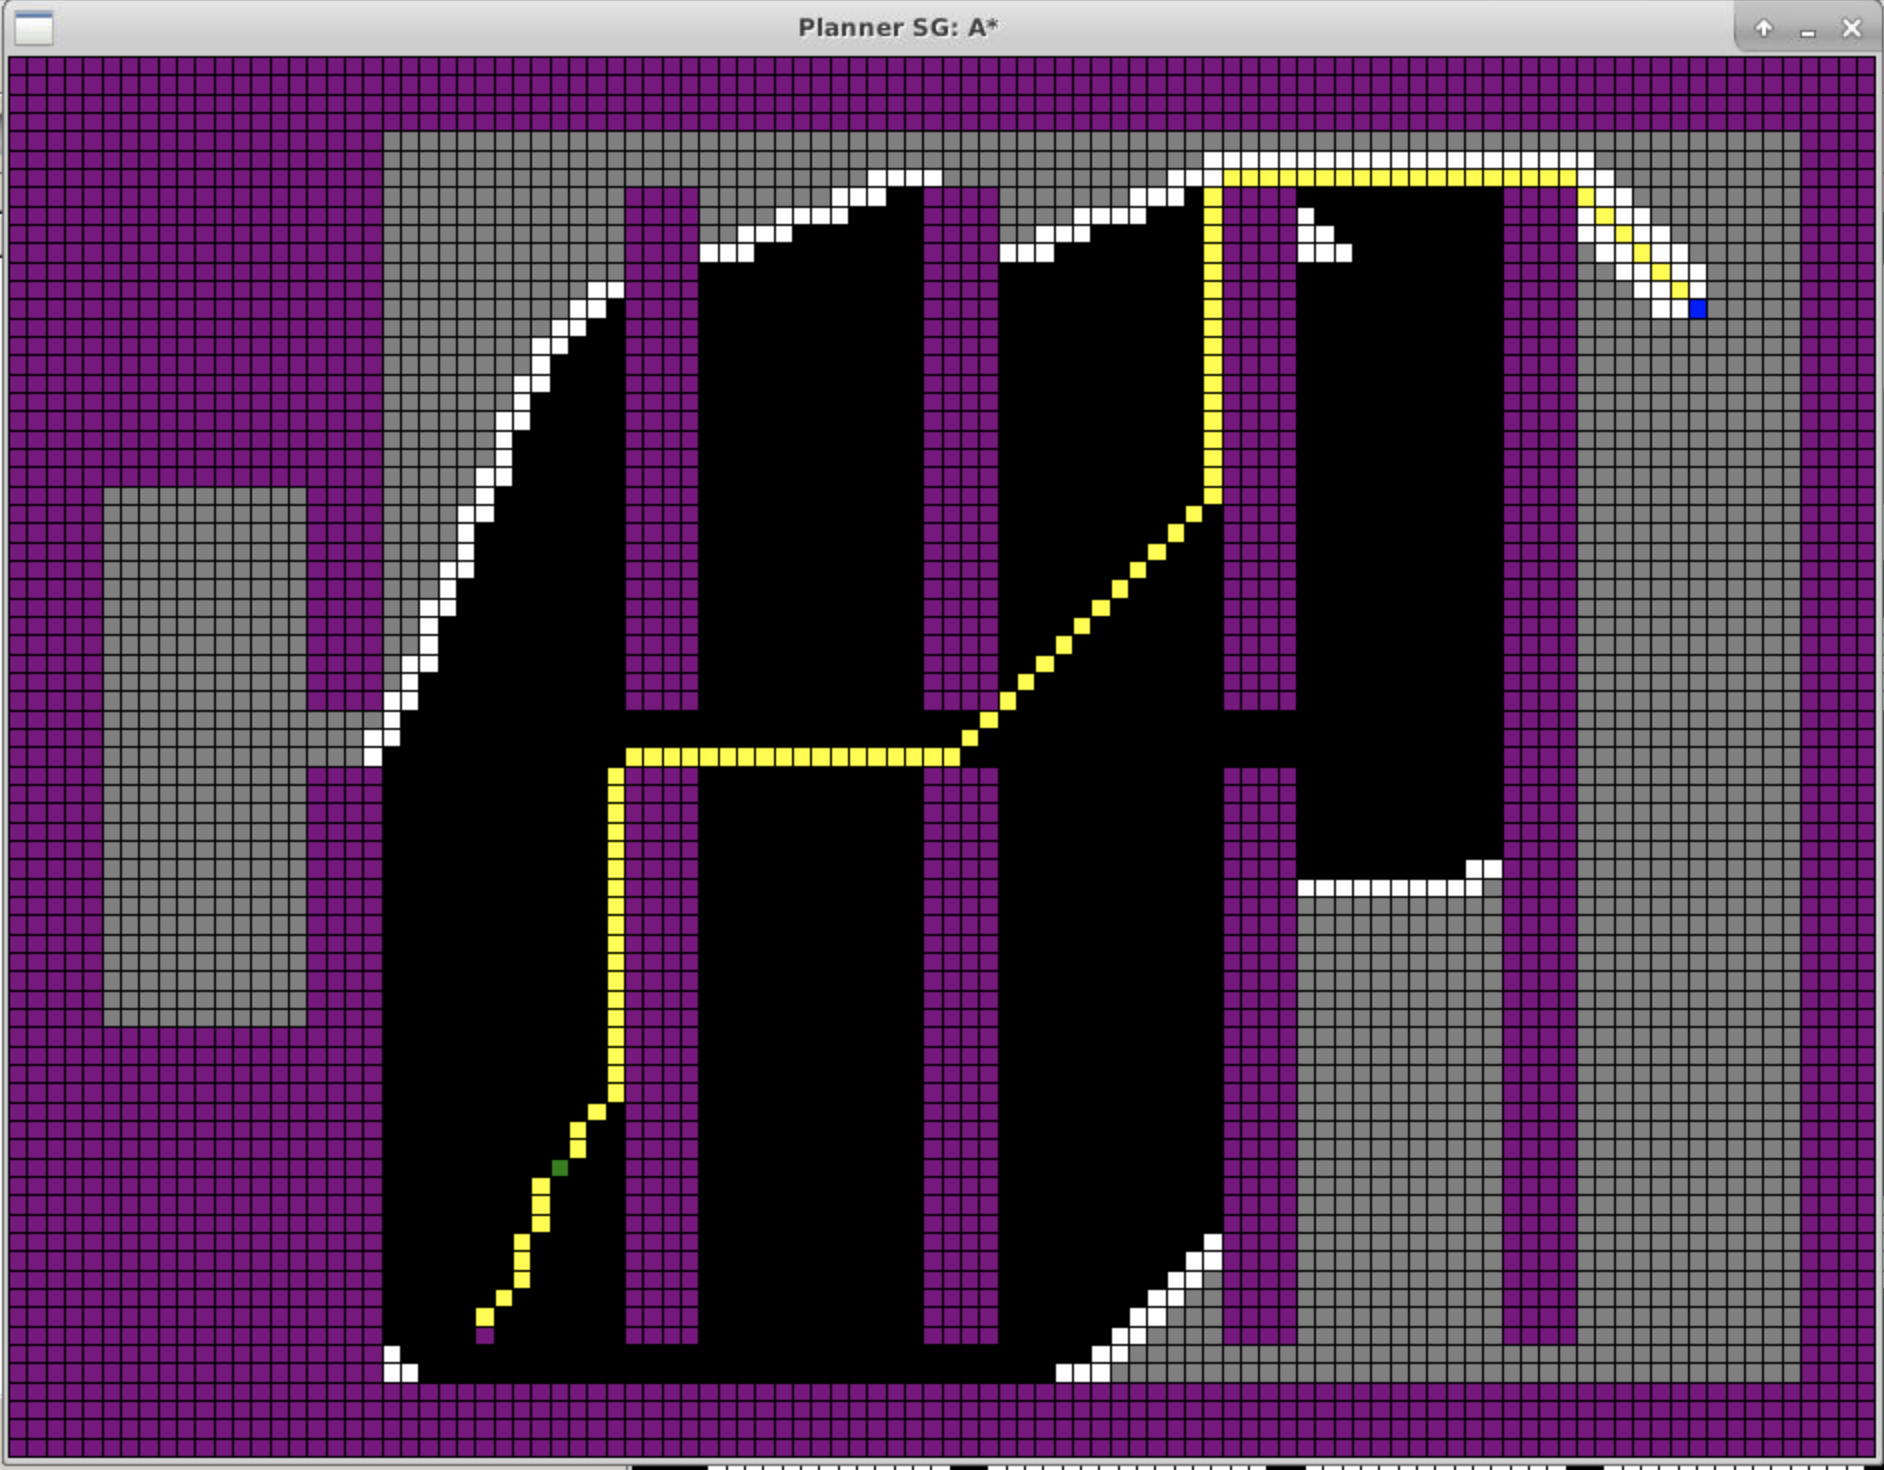
\includegraphics[width=0.32\textwidth]{graphs/part2/2-1/A.png}}
\subfigure[Via Aisle B]{
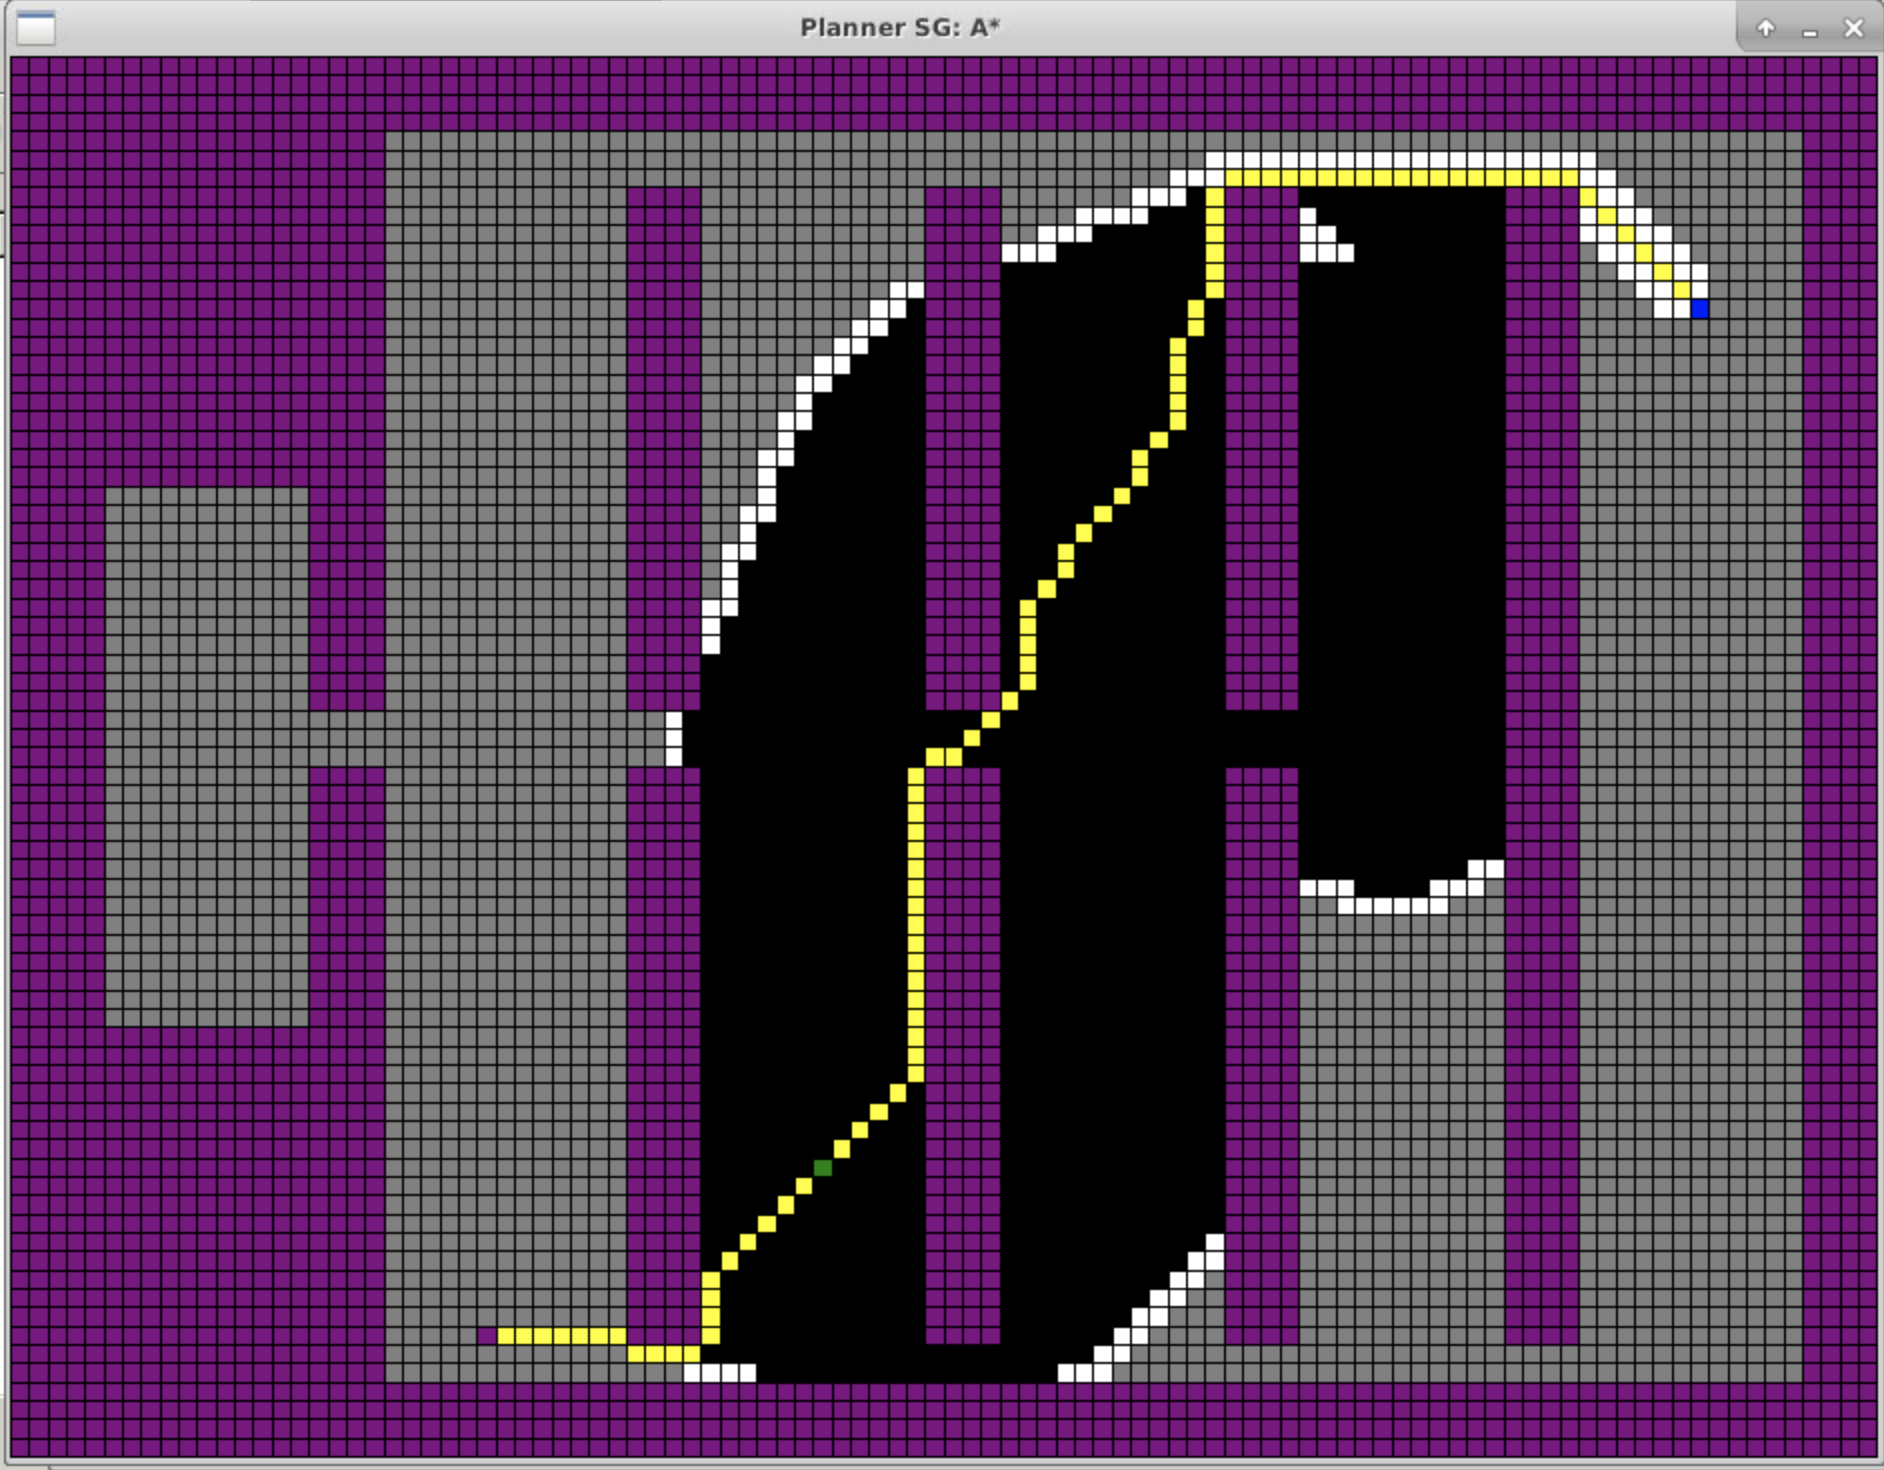
\includegraphics[width=0.32\textwidth]{graphs/part2/2-1/B.png}}
\subfigure[Via Aisle C]{
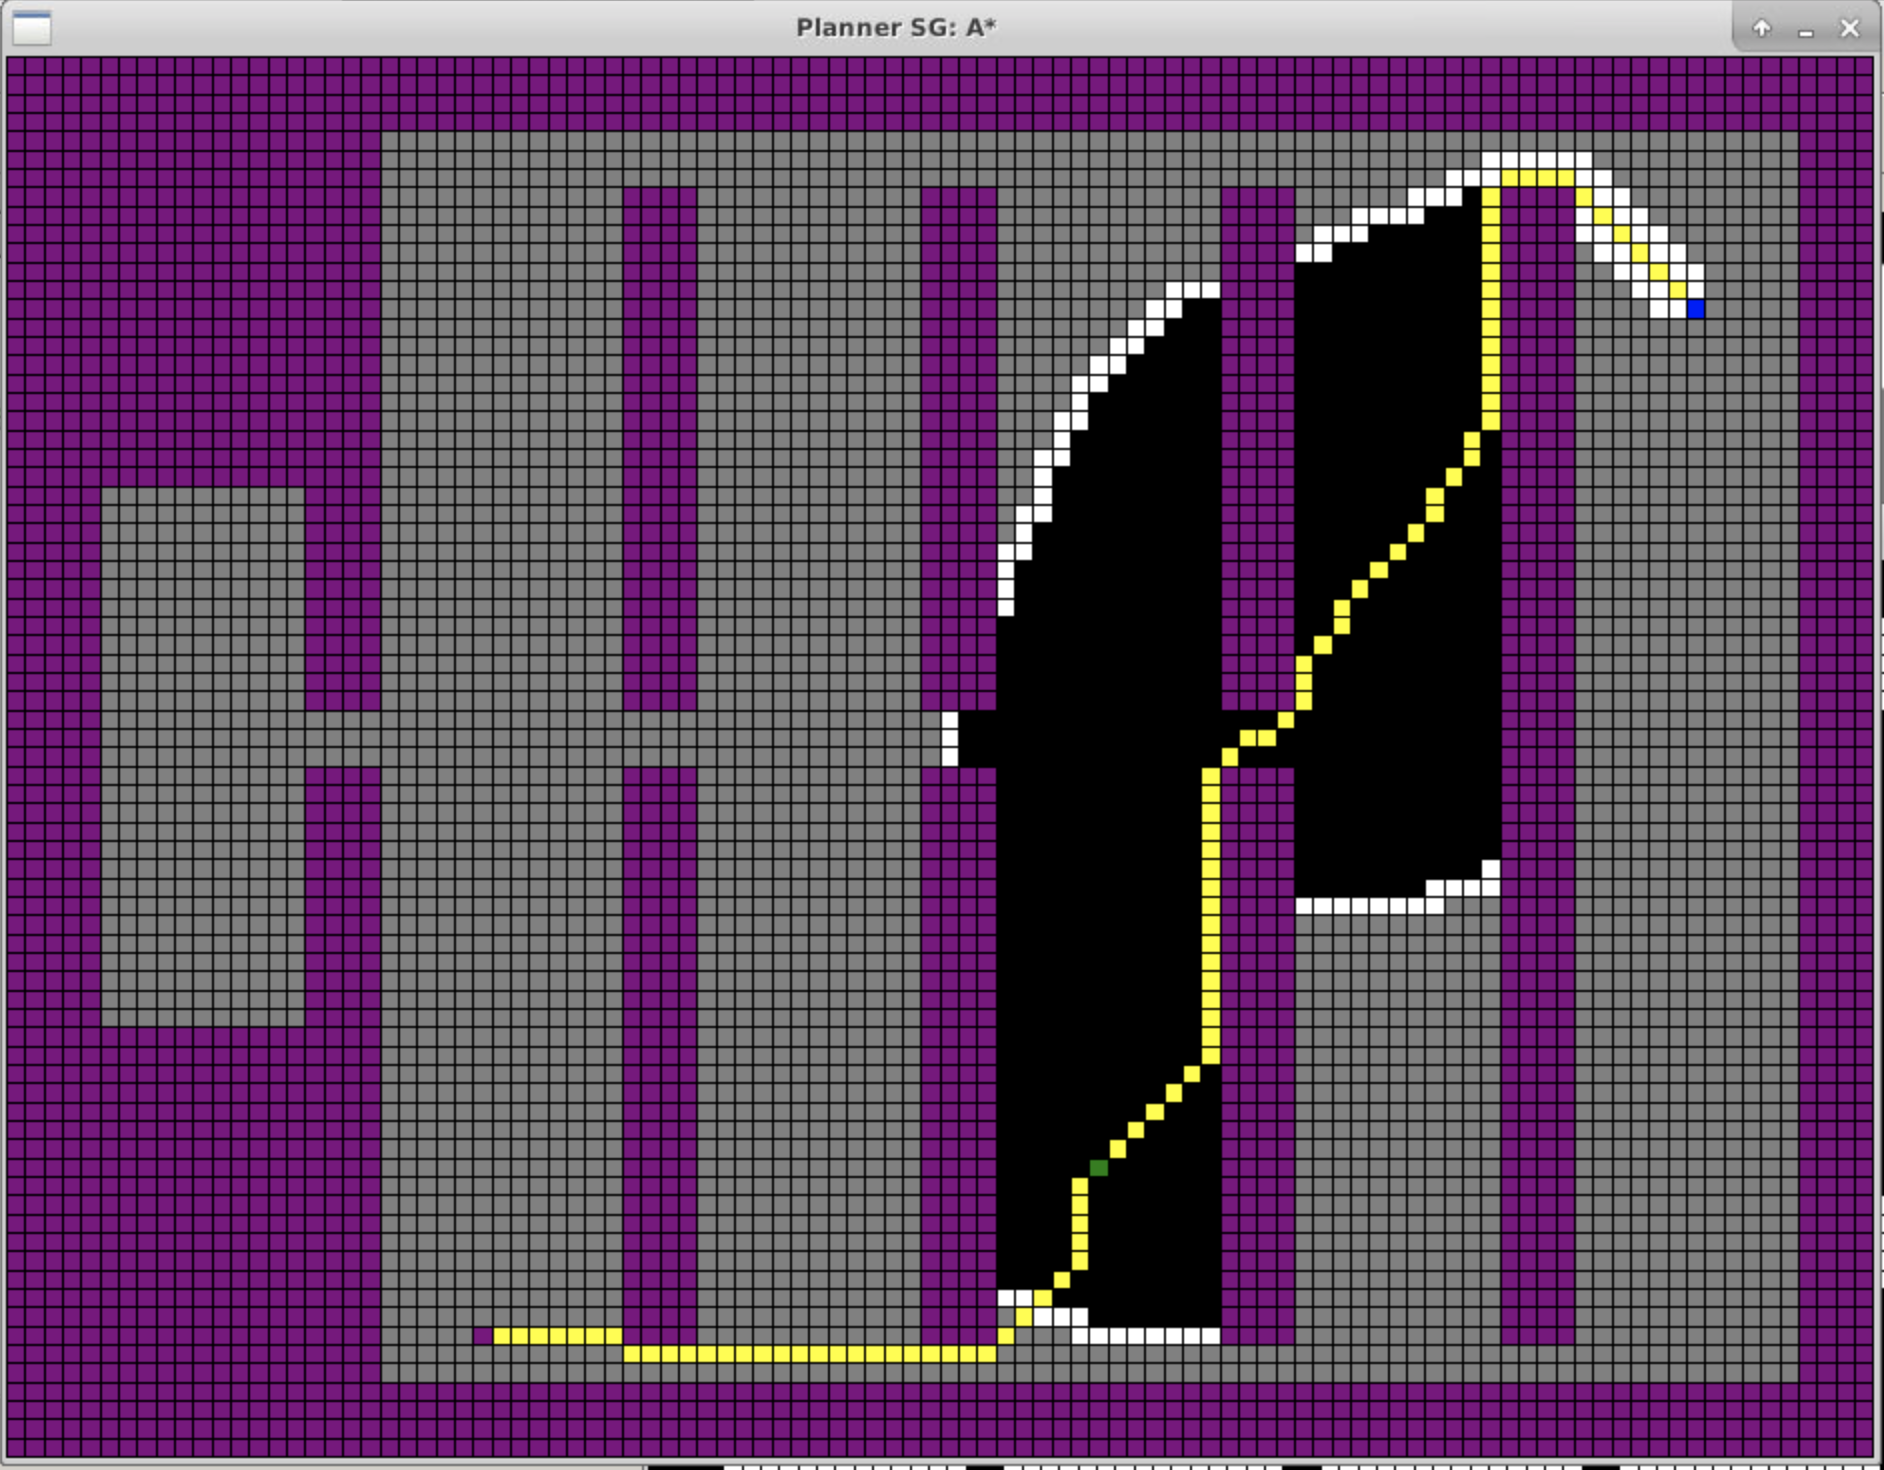
\includegraphics[width=0.32\textwidth]{graphs/part2/2-1/C.png}}
\subfigure[Via Aisle D]{
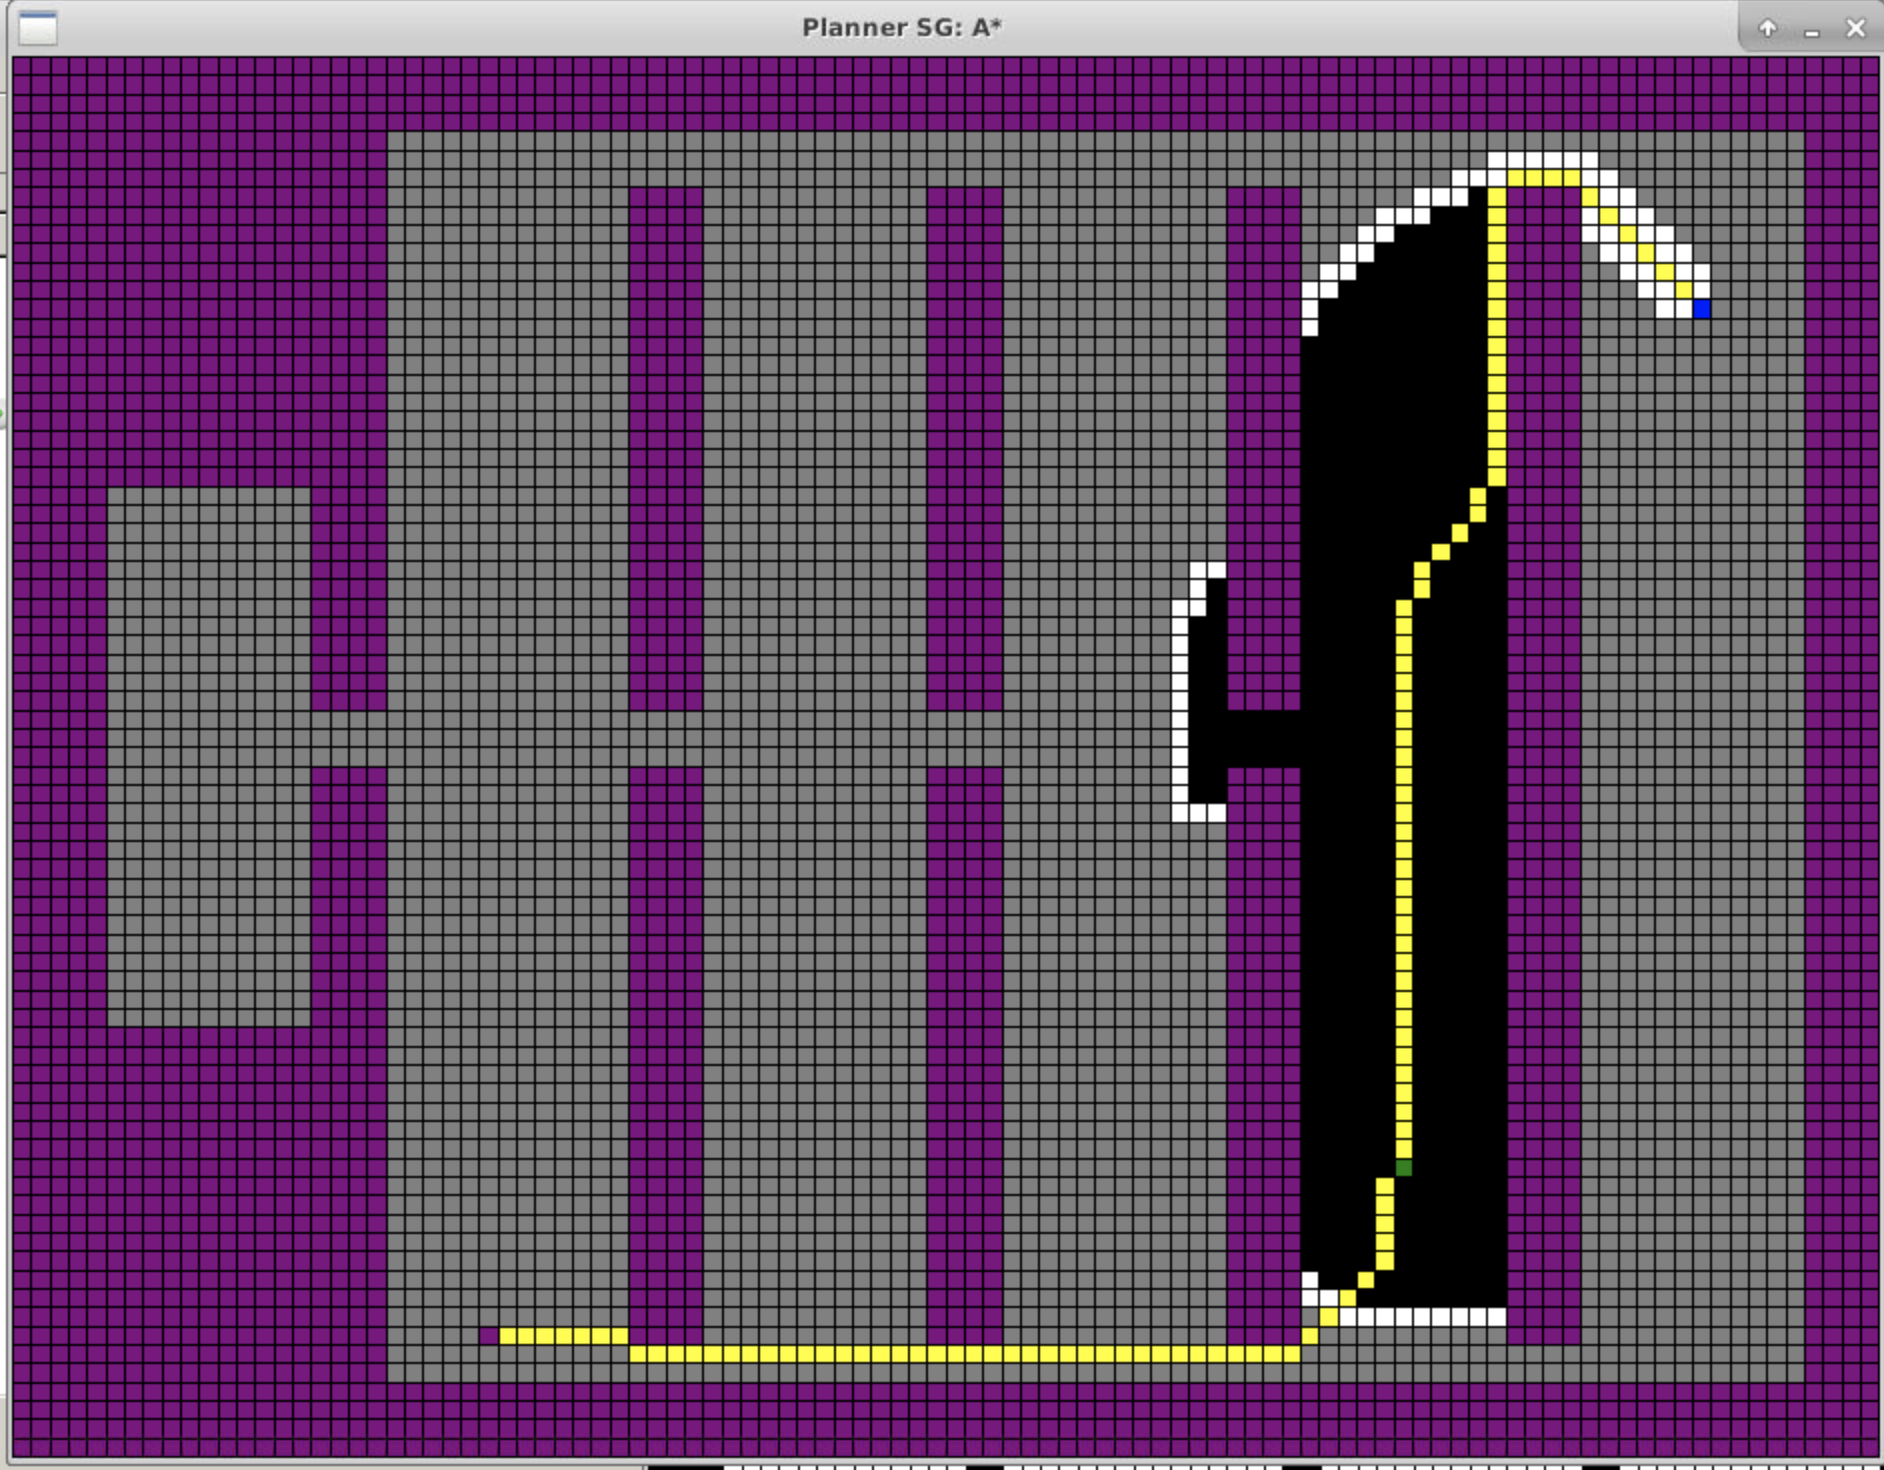
\includegraphics[width=0.35\textwidth]{graphs/part2/2-1/D.png}}
\subfigure[Via Aisle E]{
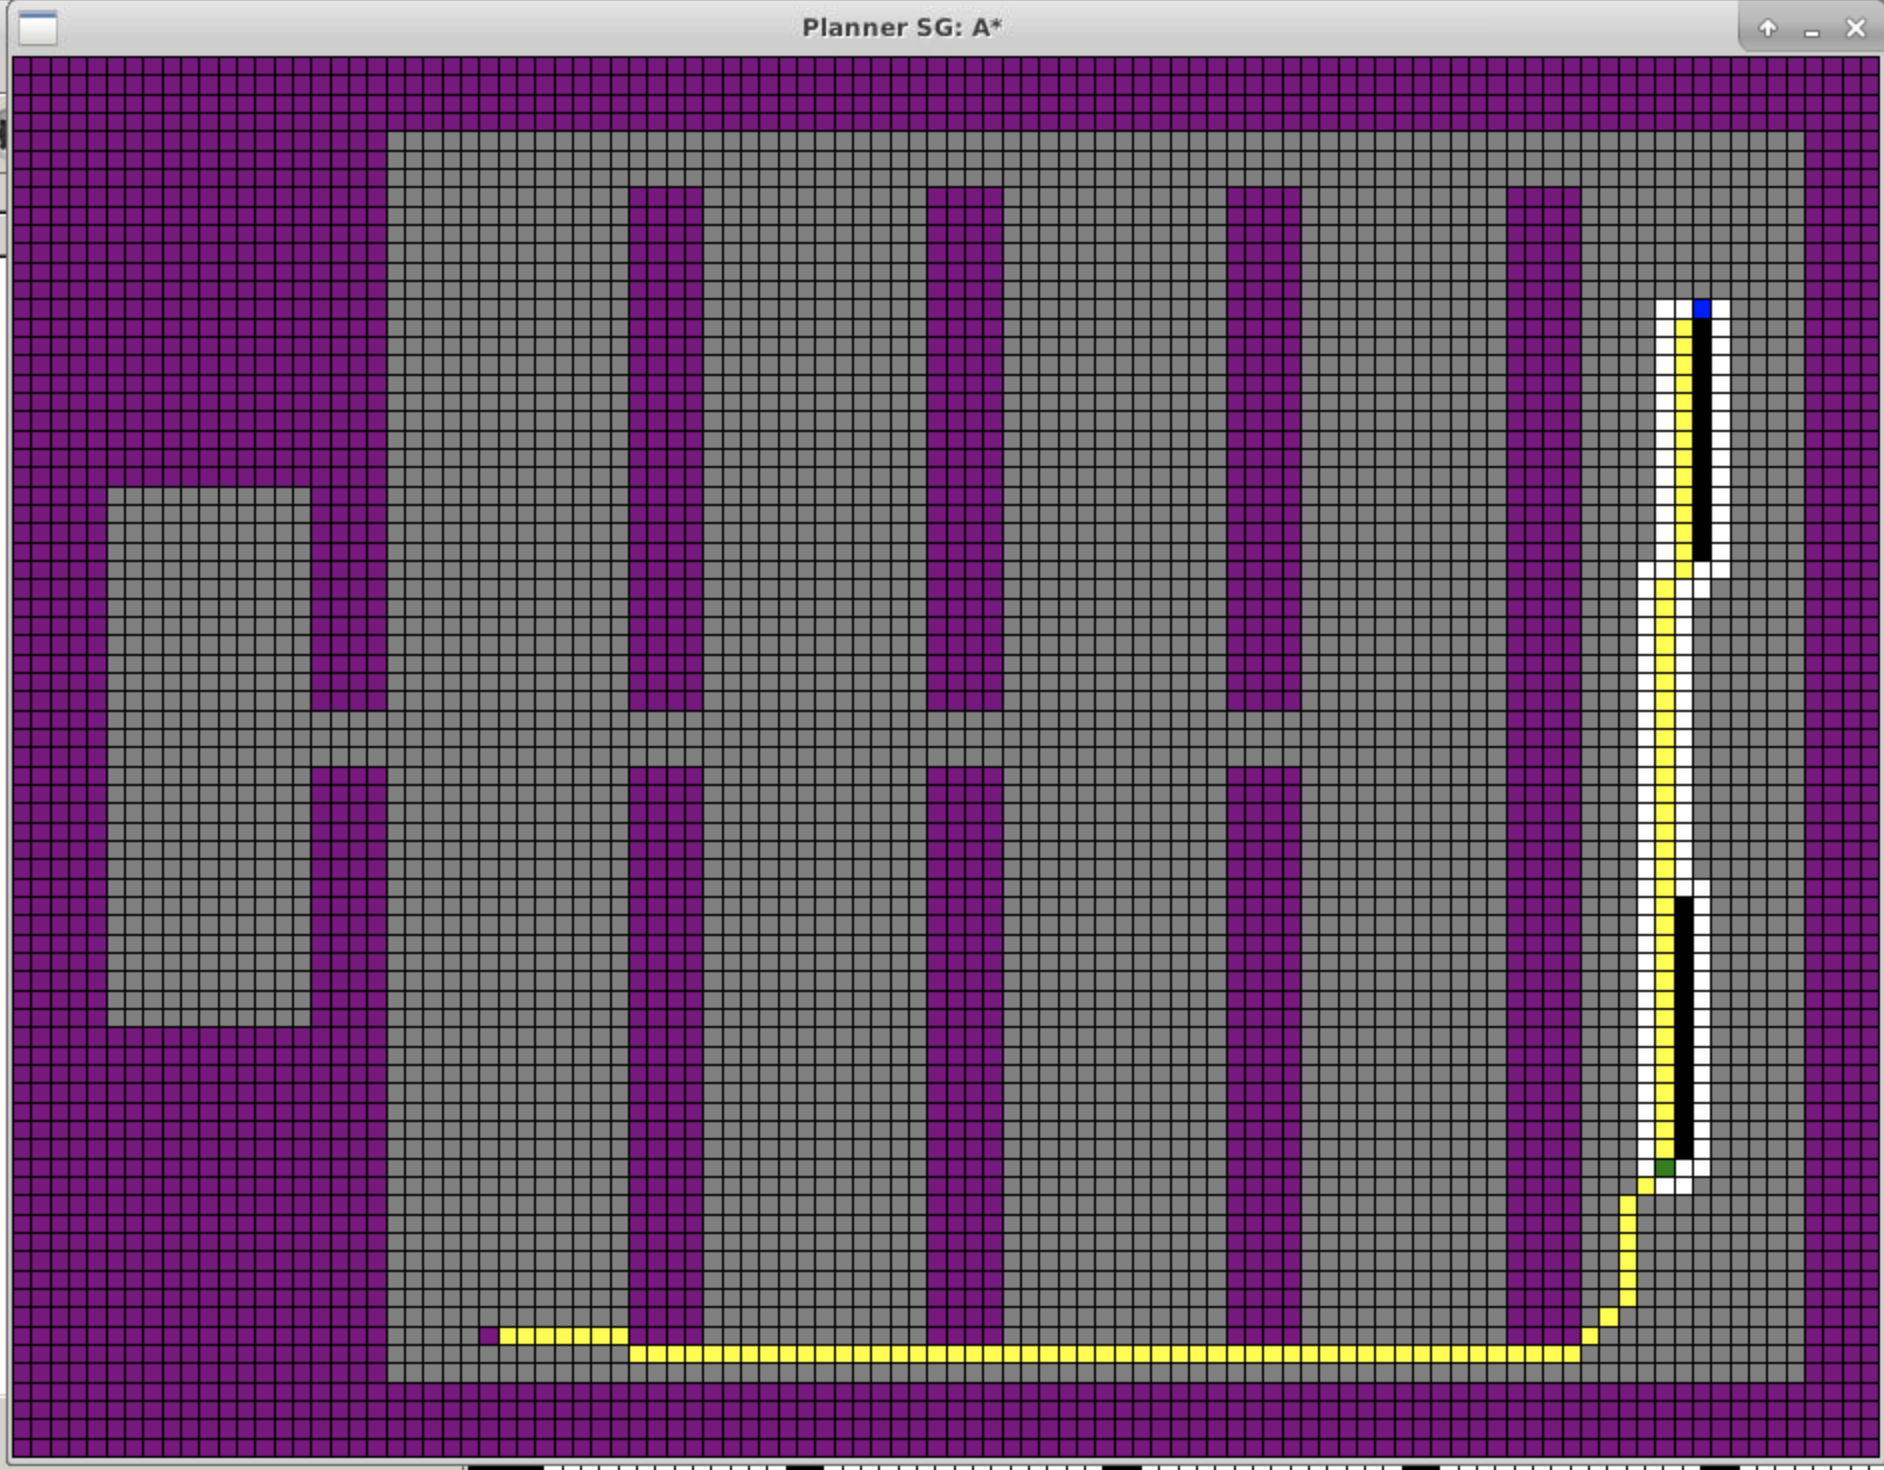
\includegraphics[width=0.35\textwidth]{graphs/part2/2-1/E.png}}
\caption{Planned Routes Down all the Different Initial Aisles}
\label{performance2.1}
\end{figure}

% ------------------
\subsection{}

We first implement the \textit{waitUntilTheObstacleClears()}. To meet the requirements we first find the obstructed cell in the current path waypoints. Then the function keeps checking the cell status with an infinite loop, and returns only if the status has been updated and became empty. 

To determine whether the robot should wait or not, we need to compute the travel cost of the remaining original path and the new planned path from the current position. For the latter we can simply use the function \textit{planPathToGoalViaAisle()} to re-plan a new path and then obtain the travel cost from the provided path property \textit{path.travelCost}. Coming to the remaining original path cost, we need to get the travel cost of the path from original start cell to current position first. Then what we want is the travel cost of the current (or original) path minus it. 

At the end of the function we calculate the threshold value of the expected $T_{W}$ (= $\frac{\text{remaining original path cost} - \text{new path cost}}{L_{W}}$) and also the corresponding $\lambda_{B}$ ($ = 1/ \mathbb{E}(T_{W})$), and output to terminal. If the $T_{W}$ we feed in is less than or equal to the threshold value, then the function \textit{shouldWaitUnitlTheObstacleToClear()} returns true.

\begin{figure}[H]
\centering  
\subfigure[Data]{
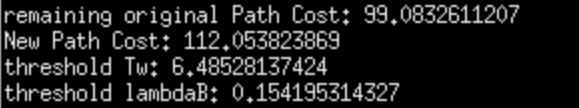
\includegraphics[width=0.5\textwidth]{graphs/part2/2-2/data.png}
\label{2-2resultData}
}
\subfigure[The search grid. The robot detects the obstacle when it reached the circled cell.]{
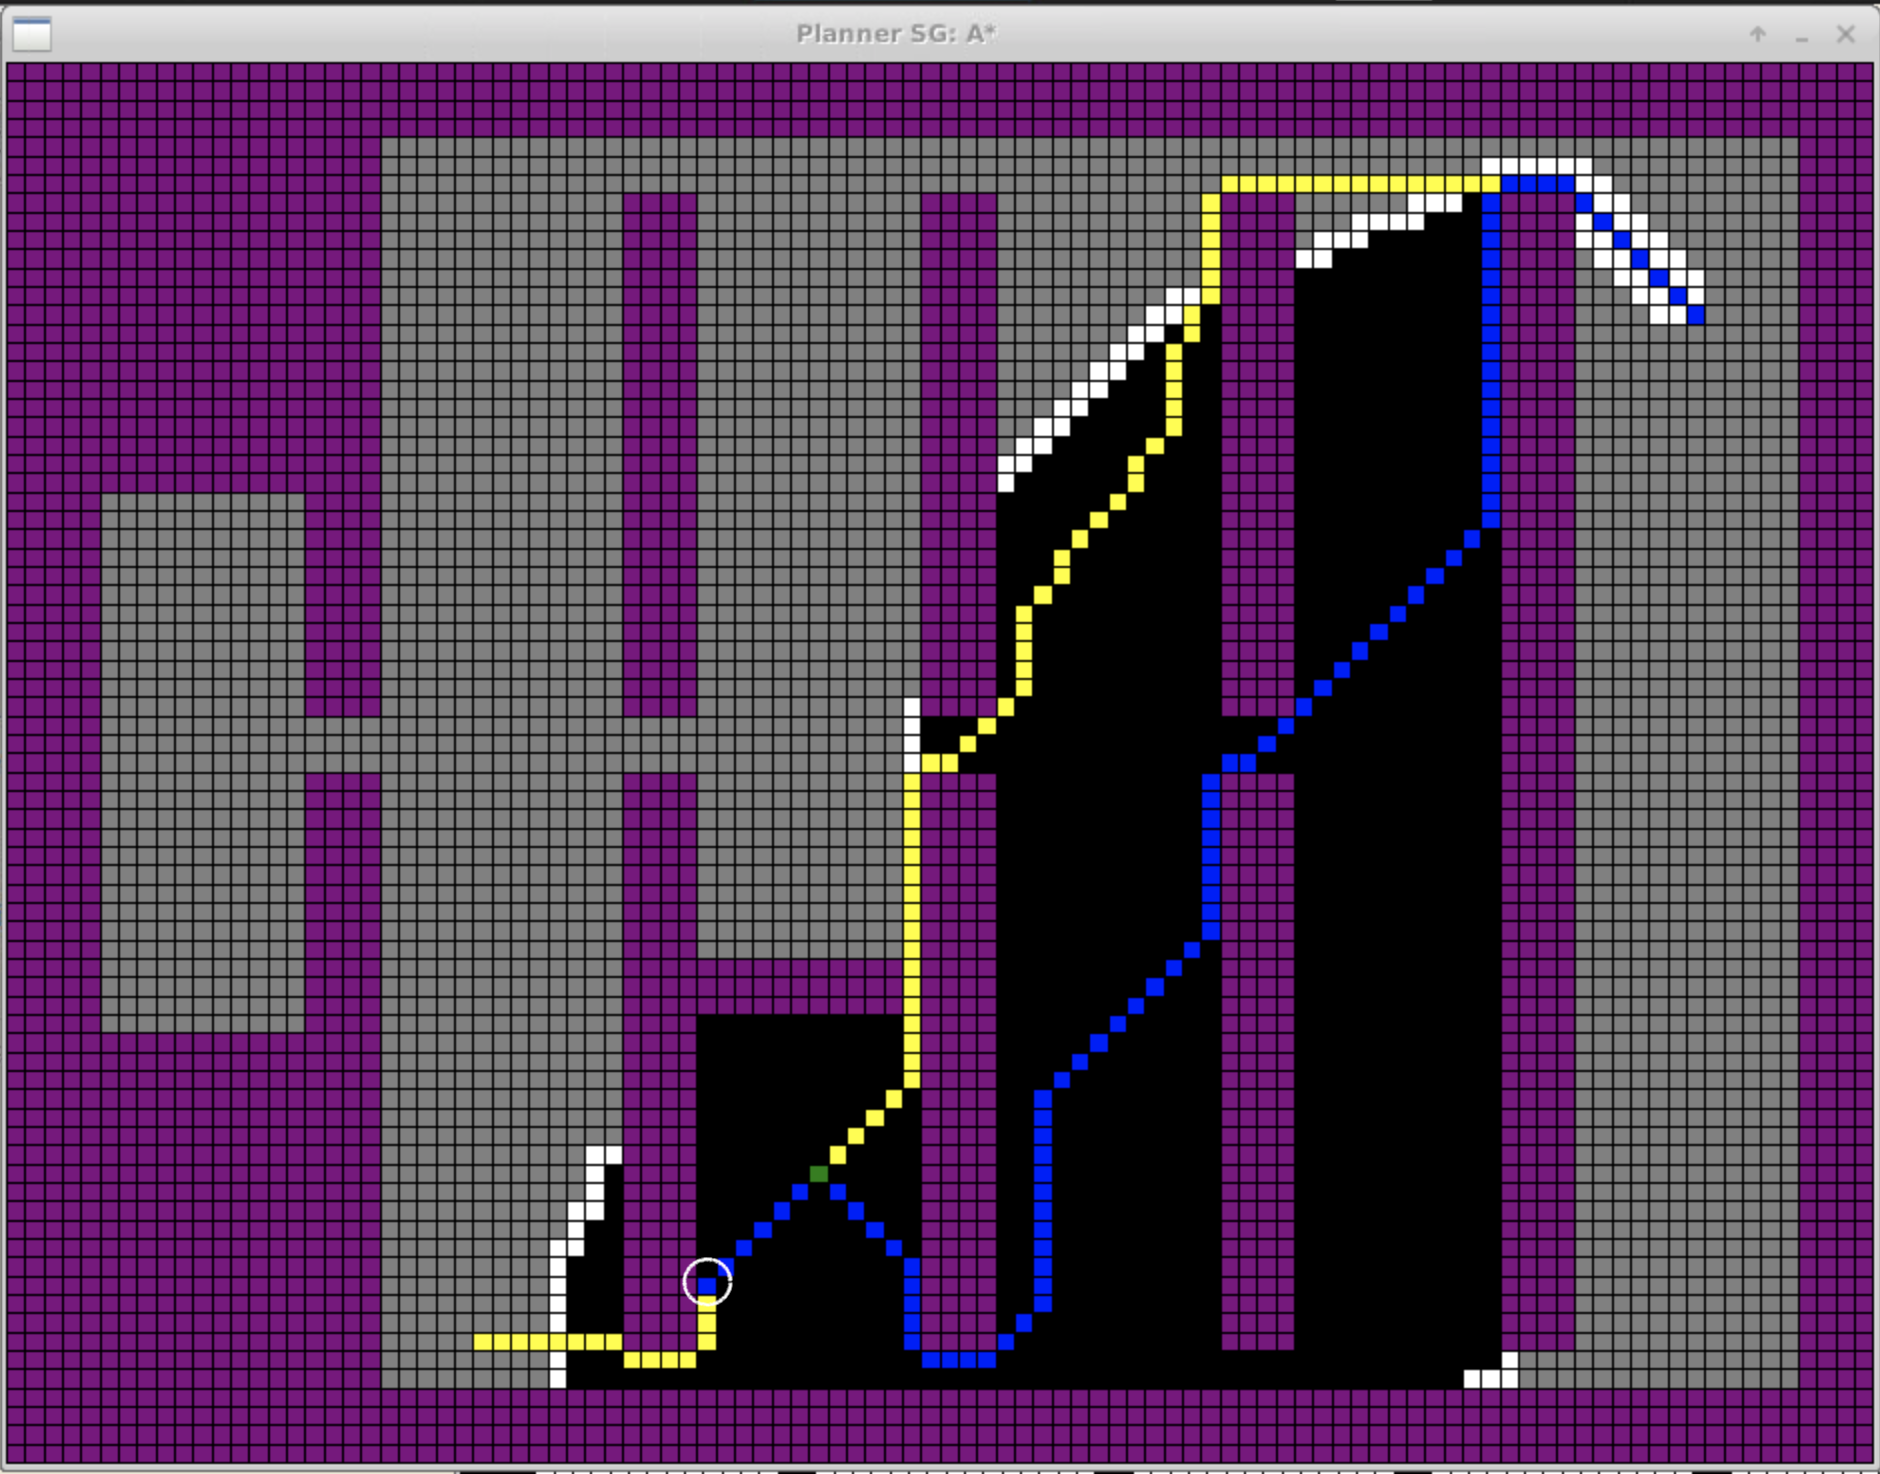
\includegraphics[width=0.7\textwidth]{graphs/part2/2-2/twoPathsSG2.png}
\label{twoPathSG}
}
\caption{Result of a single run}
\label{result2.2}
\end{figure}

Fig.\ref{result2.2} shows the result of a single run of our implementation. From the Fig.\ref{2-2resultData} we can see that the new path cost is 112.0538 while the remaining original path cost (excluding the waiting time) is 99.0833. If the wait time we feed in is less than or equal to the threshold $T_{W}$ (6.4853) then the robot will wait until the obstacle clear, else the robot will drive down aisle C. In other words, the minimum value of $T_{W}$ to make the robot move is 6.4853, and thus the maximum value of $\lambda_{B}$ below which the robot will move if it encounters the obstacle is 0.1541

% ------------------
\subsection{}

We use the function \textit{planPathToGoalViaAisle()} to plan the paths via aisle B and via aisle C. We only consider the two paths here due to that there is only a single active obstacle and it always presents in aisle B. The travel cost is obtained by using the provided path property \textit{path.travelCost}. We then calculate the threshold expected $T_{W}$ (= $\frac{\text{pathCost\_C} - \text{pathCost\_B}}{L_{W}}$) and the corresponding $\lambda_{B}$ ($ = p/ \mathbb{E}(T_{W})$) and output the values to terminal. With the threshold values, the waiting time is then input by users from terminal to determine which path the robot will choose. If the waiting time greater than or equal to the threshold value then the robot will go down the aisle C.

\begin{figure}[H]
\centering  
\subfigure[Data]{
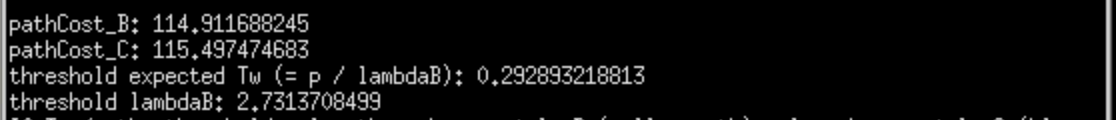
\includegraphics[width=0.7\textwidth]{graphs/part2/2-3/data.png}
\label{2-3resultData}
}
\subfigure[The search grid. The yellow path is the path via aisle B, and the blue one is via aisle C.]{
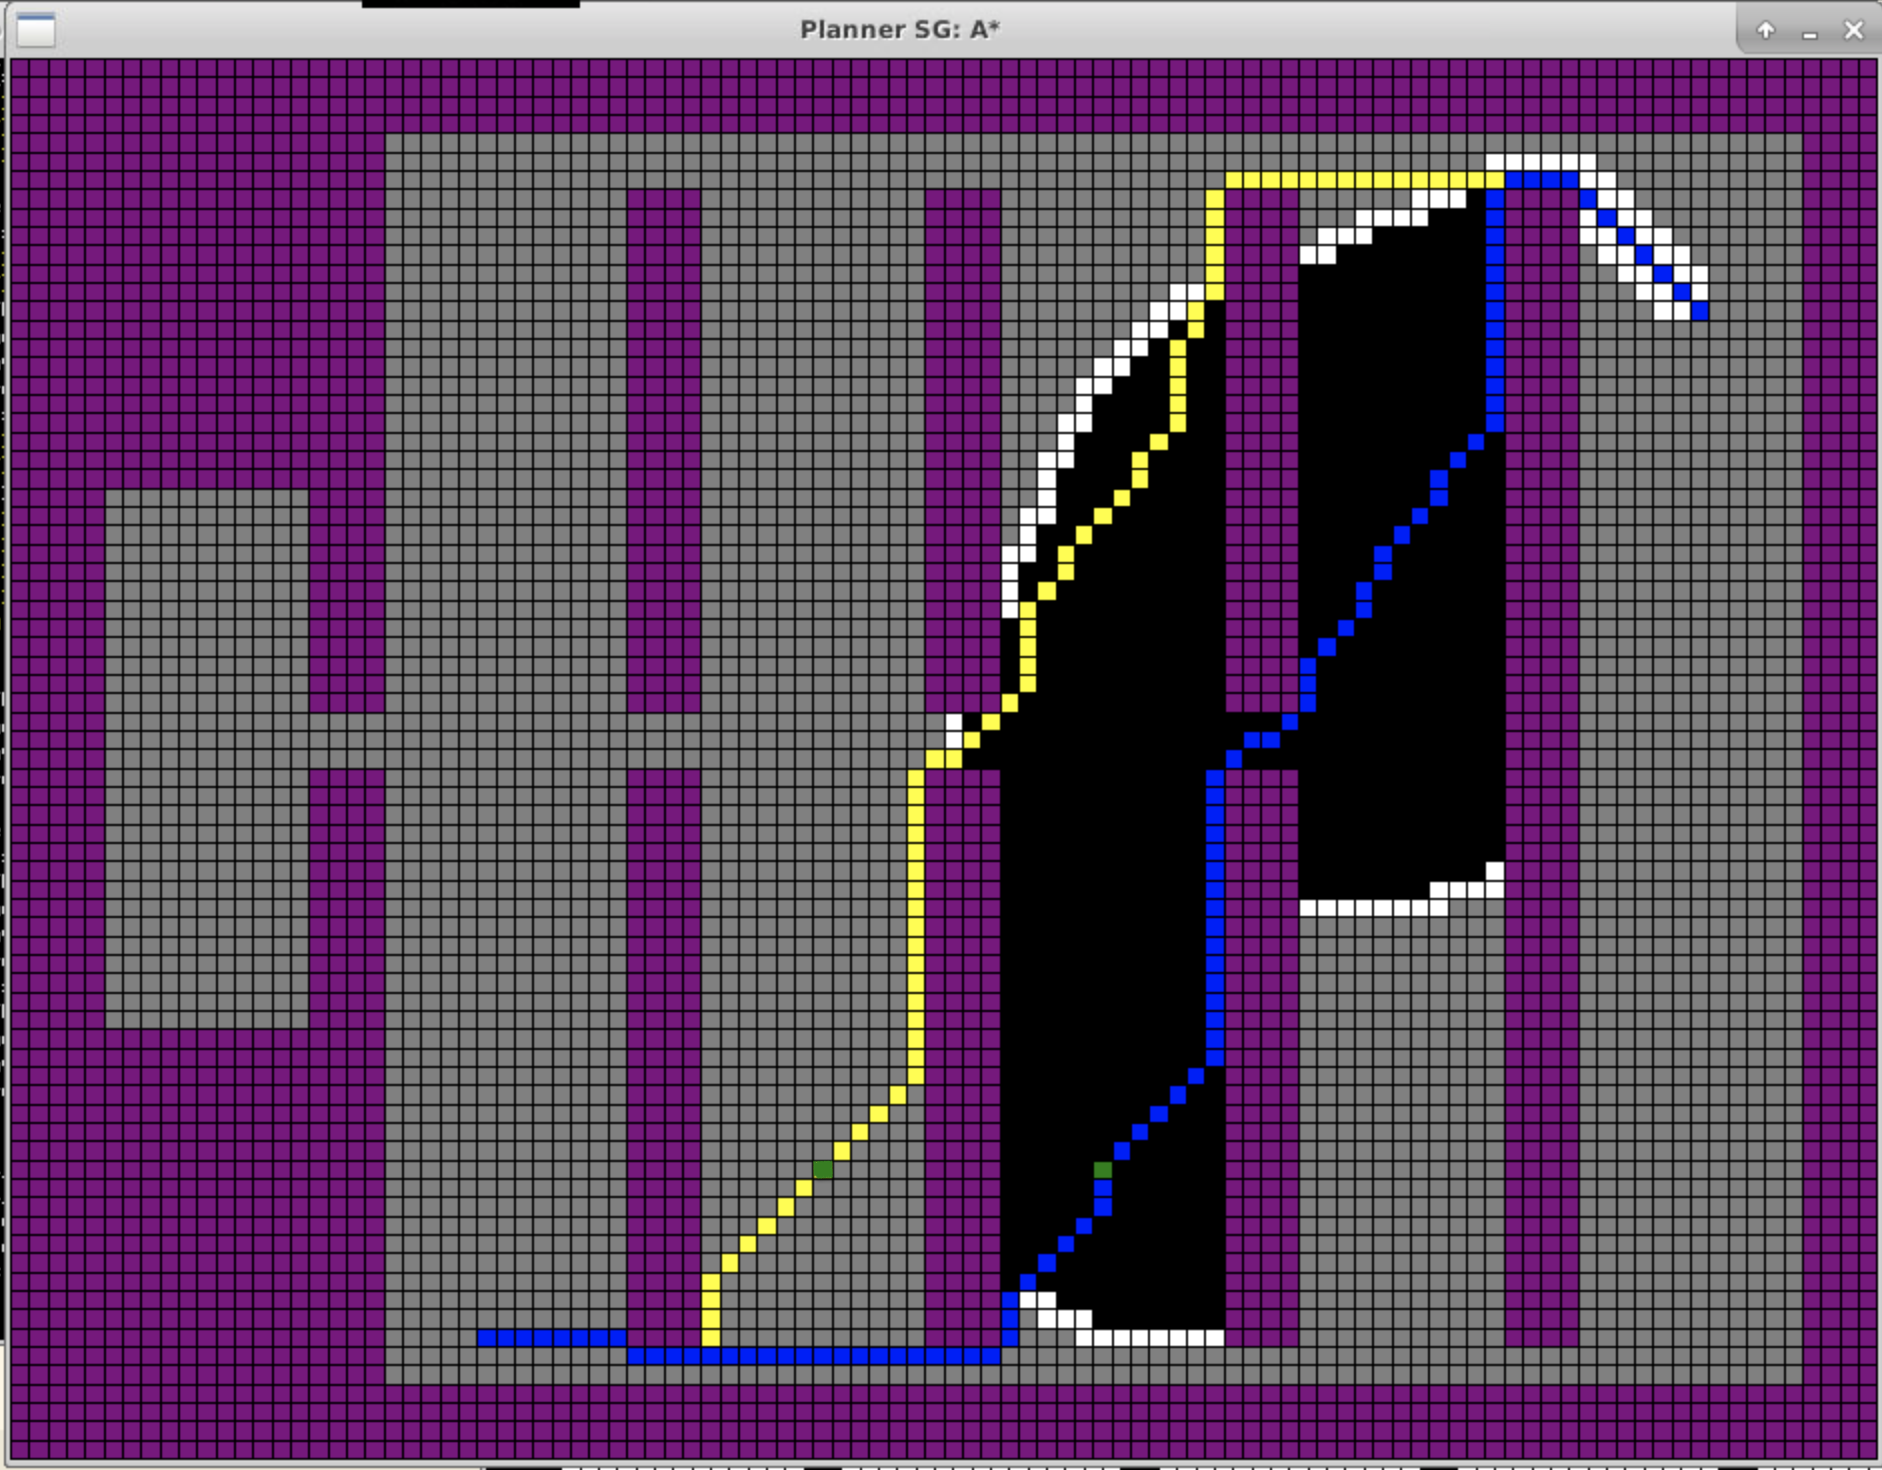
\includegraphics[width=0.7\textwidth]{graphs/part2/2-3/SG.png}
\label{2-3SG}
}
\caption{Result of a single run of our implementation}
\label{result2.3}
\end{figure}

Fig.\ref{2-3resultData}  shows the values of travel cost of the two paths of a single run(excluding the waiting cost if it encounters an obstacle at aisle B) and the values of the threshold of the waiting-time-related parameters. There is little difference between the travel cost of the two paths if we do not take the waiting time into consider. The threshold expected $T_{W}$ tells that if the waiting time is greater than or equal to 0.2928, then the robot will go directly down aisle C. So the maximum value of $\lambda_{B}$ is 2.7313.

\newpage


% -----------------------------------------------------------------------------------------
\end{document}